%%%%%%%%%%%%%%%%%%%%%%%%%%%%%%%
%This is the article LaTeX template for RSC journals
%Copyright The Royal Society of Chemistry 2010
%%%%%%%%%%%%%%%%%%%%%%%%%%%%%%%


\documentclass[8.5pt,twoside,twocolumn]{article}
\oddsidemargin -1.2cm
\evensidemargin -1.2cm
\textwidth 18cm
\headheight 1.0in
\topmargin -3.5cm
\textheight 22cm
\usepackage[super,sort&compress,comma]{natbib} 
\usepackage{mhchem}
\usepackage[utf8]{inputenc}
\usepackage{times,mathptmx}
% \usepackage{times}
% feel free not to use mathptmx if it causes difficulties
\usepackage{sectsty}
\usepackage{balance} 

\usepackage{graphicx} %eps figures can be used instead
\usepackage{lastpage}
\usepackage[format=plain,justification=raggedright,singlelinecheck=false,font=small,labelfont=bf,labelsep=space]{caption} 
\usepackage{fancyhdr}
\pagestyle{fancy}

\begin{document}

\thispagestyle{plain}
\fancypagestyle{plain}{
\fancyhead[L]{
\includegraphics[height=8pt]{headers/LH}}
\fancyhead[C]{\hspace{-1cm}
\includegraphics[height=20pt]{headers/CH}}
\fancyhead[R]{
\includegraphics[height=10pt]{headers/RH}\vspace{-0.2cm}}
\renewcommand{\headrulewidth}{1pt}}
\renewcommand{\thefootnote}{\fnsymbol{footnote}}
\renewcommand\footnoterule{\vspace*{1pt}% 
\hrule width 3.4in height 0.4pt \vspace*{5pt}} 
\setcounter{secnumdepth}{5}



\makeatletter 
\def\subsubsection{\@startsection{subsubsection}{3}{10pt}{-1.25ex plus -1ex minus -.1ex}{0ex plus 0ex}{\normalsize\bf}} 
\def\paragraph{\@startsection{paragraph}{4}{10pt}{-1.25ex plus -1ex minus -.1ex}{0ex plus 0ex}{\normalsize\textit}} 
\renewcommand\@biblabel[1]{#1}            
\renewcommand\@makefntext[1]% 
{\noindent\makebox[0pt][r]{\@thefnmark\,}#1}
\makeatother 
\renewcommand{\figurename}{\small{Fig.}~}
\sectionfont{\large}
\subsectionfont{\normalsize} 

\fancyfoot{}
\fancyfoot[LO,RE]{\vspace{-7pt}
\includegraphics[height=9pt]{headers/LF}}
\fancyfoot[CO]{\vspace{-7.2pt}\hspace{12.2cm}
\includegraphics{headers/RF}}
\fancyfoot[CE]{\vspace{-7.5pt}\hspace{-13.5cm}
\includegraphics{headers/RF}}
\fancyfoot[RO]{\footnotesize{\sffamily{1--\pageref{LastPage} ~\textbar  \hspace{2pt}\thepage}}}
\fancyfoot[LE]{\footnotesize{\sffamily{\thepage~\textbar\hspace{3.45cm} 1--\pageref{LastPage}}}}
\fancyhead{}
\renewcommand{\headrulewidth}{1pt} 
\renewcommand{\footrulewidth}{1pt}
\setlength{\arrayrulewidth}{1pt}
\setlength{\columnsep}{6.5mm}
\setlength\bibsep{1pt}

\twocolumn[
  \begin{@twocolumnfalse}
\noindent\LARGE{\textbf{Oscillations in CO-oxidation Catalysts at Atmospheric Pressures$^\dag$}}
\vspace{0.6cm}

\noindent\large{\textbf{Robert Jensen\textit{$^{b}$}, Thomas Andersen\textit{$^{b}$}, Anders Nierhoff\textit{$^{b}$}, Søren Dahl\textit{$^{b}$}, Ole Hansen\textit{$^{b}$} and Ib Chorkendorff\textit{$^{a}$}}}\vspace{0.5cm}
%Please note that \ast indicates the corresponding author(s) but no footnote text is required. 


\noindent\textit{\small{\textbf{Received Xth XXXXXXXXXX 20XX, Accepted Xth XXXXXXXXX 20XX\newline
First published on the web Xth XXXXXXXXXX 200X}}}

\noindent \textbf{\small{DOI: 10.1039/b000000x}}
\vspace{0.6cm}
%Please do not change this text.

\noindent \normalsize{The abstract should be a single paragraph which summarises the content of the article. Any references in the abstract should be written out in full \textit{e.g.} [Surname \textit{et al., Journal Title}, 2000, \textbf{35}, 3523].}
\vspace{0.5cm}
 \end{@twocolumnfalse}
  ]


%\section{This is the section heading style}
\section{Introduction}

%Footnotes
\footnotetext{\dag~Electronic Supplementary Information (ESI) available: [details of any supplementary information available should be included here]. See DOI: 10.1039/b000000x/}

%Please use \dag to cite the ESI in the main text of the article.
%If you article does not have ESI please remove the the \dag symbol from the title and the above footnotetext.

\footnotetext{\textit{$^{a}$~DTU Physics, Fysikvej 312, 2800 Lyngby, Denmark. Fax: XX XXXX XXXX; Tel: XX XXXX XXXX; E-mail: ibchork@fysik.dtu.dk}}
\footnotetext{\textit{$^{b}$~DTU Physics, Fysikvej 312, 2800 Lyngby, Denmark}}

%additional addresses can be cited as above using the lower-case letters, c, d, e... If all authors are from the same address, no letter is required

%\footnotetext{\ddag~Additional footnotes to the title and authors can be included \emph{e.g.}\ `Present address:' or `These authors contributed equally to this work' as above using the symbols: \ddag, \textsection, and \P. Please place the appropriate symbol next to the author's name and include a \texttt{\textbackslash footnotetext} entry in the the correct place in the list.}

Oxidation of CO is a classic model system for testing catalytic properties of various materials. It was shown already in 1985 (REF) that this reaction will show oscilaltory behaviour under UHV conditions due to surface reconstructions having large influence on the catalytic activity of the surface. However, this is a phenomenon that is only observed under UHV-condition, under higher pressures these kinds of reconstructions will happen. In this paper we show sustained catalytic oscilations on Platinum nano particles that due to their sometimes extremely long time-scales cannot be a surface phenomenon, but must involve a bulk oxidation of the nanoparticle. 
Similar phenomeon of oscillations of CO oxidation Pt has been seen earlier on thin-films \cite{Lund2000}, single crystals \cite{Hendriksen2005} and in macroscopic flow-reactors \cite{Singh2010}, but to our knowledge never before on nano particles.

\section{Experimental Methods}
The measurents are done in a silicon-fabricated microreactor, developed here at CINF \cite{Henriksen2009}. The reactor consists of a two inlets, a long mixing zone for the incoming gases and a reactor of total volume of $240\,$nL. The reactor is able to operate at a pressure range og 0-2.5\,bar. The gases is supplied through ordinary flow controllers capable of controlling flow in the range of a few mL/min. The flow is reduced to a value capable of being fed into a mass-spectrometer by passing most of the flow through an outlet connected to a pressure controller. A small part of the flow is led into the reactor chamber and via a $5.4\,\mu$m wide capillary further into UHV chamber equiped with a quadropole mass spectrometer. The design ensures that all gas exposed to the catalyst under investigation is also measured in the mass spectrometer ensures a very high sensitivity of the device. When an evacuated microreactor is mounted, the base pressure of the UHV chambe is $\sim5\times10^{-9}\,$mbar and when operating at $1\,$bar in the reactor the pressure is $\sim5\times10^{-7}\,$mbar.

The reactor is heated by a Pt heating element evaporated on the backside that at the same time acts as an RTD to measure the temperature. 

\section{Sample preparation}
The samples was made by depositing a very small amount of size-selcted clusters from a quadropole cluster source (REF!) onto the microreactores. Typical sizes are in the order of 3-9\,nm and the coverage is kept at approximately 0.1\% geometric coverage, found by measuring the current from the charged clusters landing on the reactor. After deposition the reactor is anonicly bonded to a pyrex lid while keeping the reactor area cold by mounting the reactor on a cooling block and heating the rest of the sample to $\sim350\,^\circ$C \cite{Vesborg2010}

\section{Results}
The experiments was carried out ....

The period of the oscillations ranges from a few seconds (the time-constant of the reactor) up to more than an hour. A typical slow is oscillation is seen in figure~\ref{fgr:full_oscillation} where we see the typical pattern going from almost no activity slowly up towards $\sim$50\% conversion at which point the sample light off to full conversion almost instantiously where after a short peiod of time the sample again de-activates.
% an example of a two-column figure, remember that the graphics should be included where it is first referenced
\begin{figure*}
  \centering
  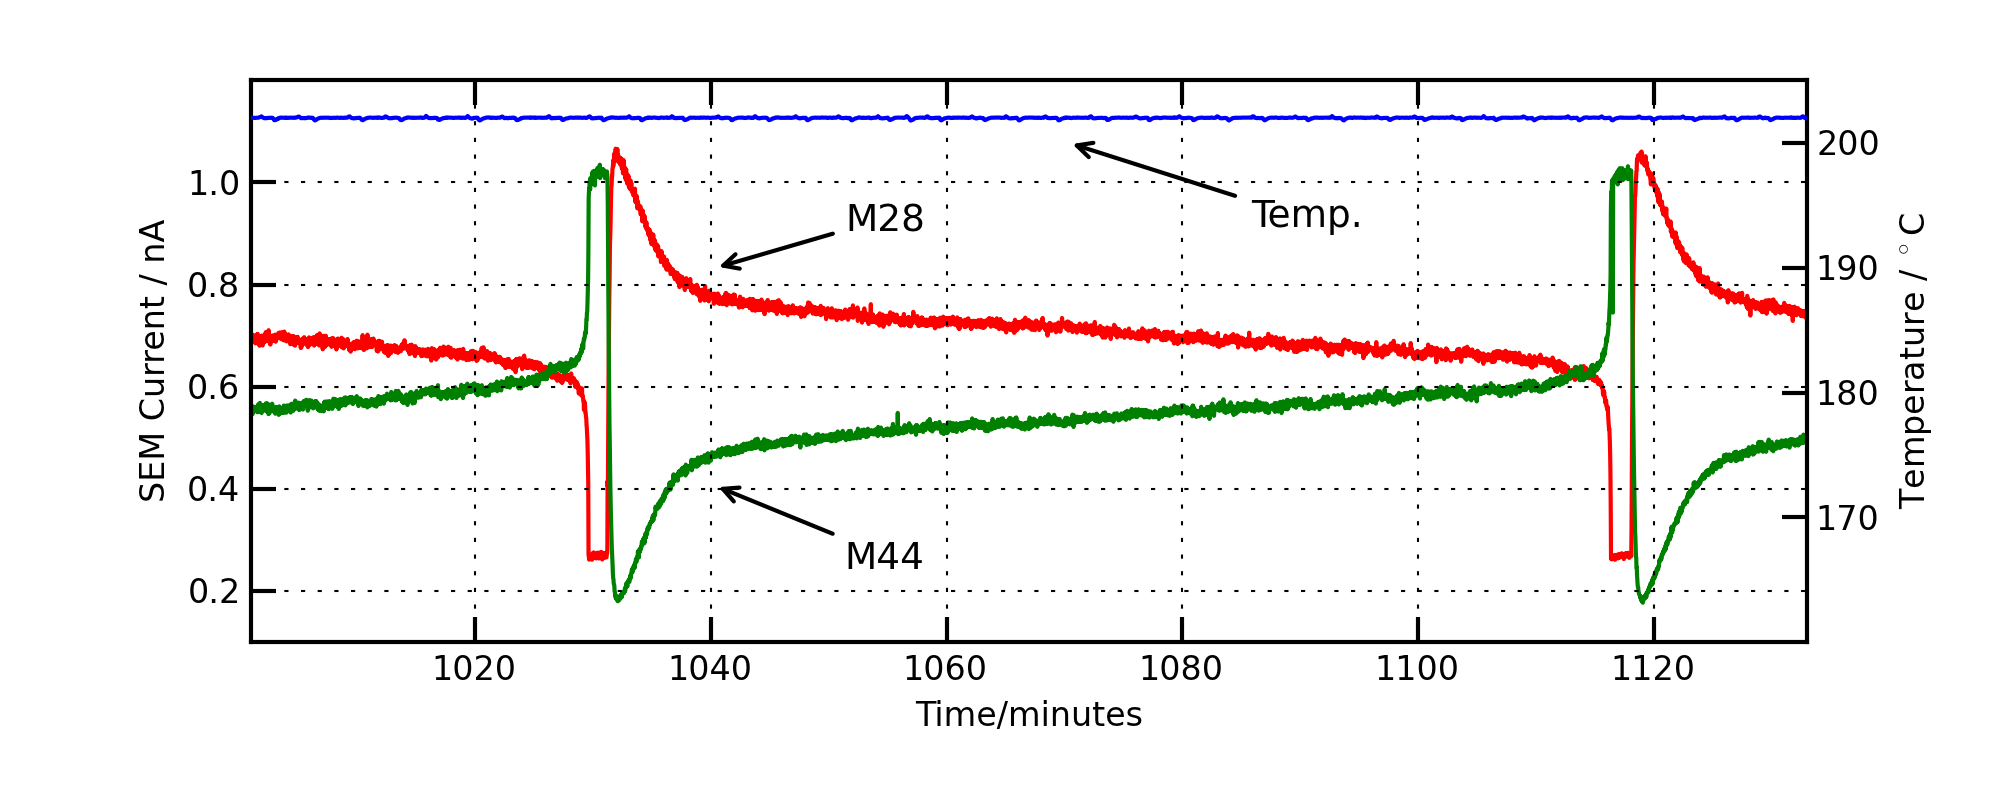
\includegraphics[height=7cm]{single_full_oscillation.png}
  \caption{A full oscillation first showing a steep ignition of the sample followed by an almost imidiately de-activation of the sample. For the next 65\,minutes the sample slowly recovers activity until it again lights off completely.}
  \label{fgr:full_oscillation}
\end{figure*}

If a sample is leaved for long periods of time, it keep performing sustained oscillations, but with longer and longer periods. In the beginning the period is very stable and sligtly increasing but after a few days, the periods becomes more and more noisy although still maintaining the trend of longer and longer periods. Figure~\ref{fgr:full_oscillation} shows a summary of the periods of a sample oscillating for 4 days. 
% an example of a single-column figure, remember that the graphics should be included where it is first referenced
\begin{figure}[h]
\centering
  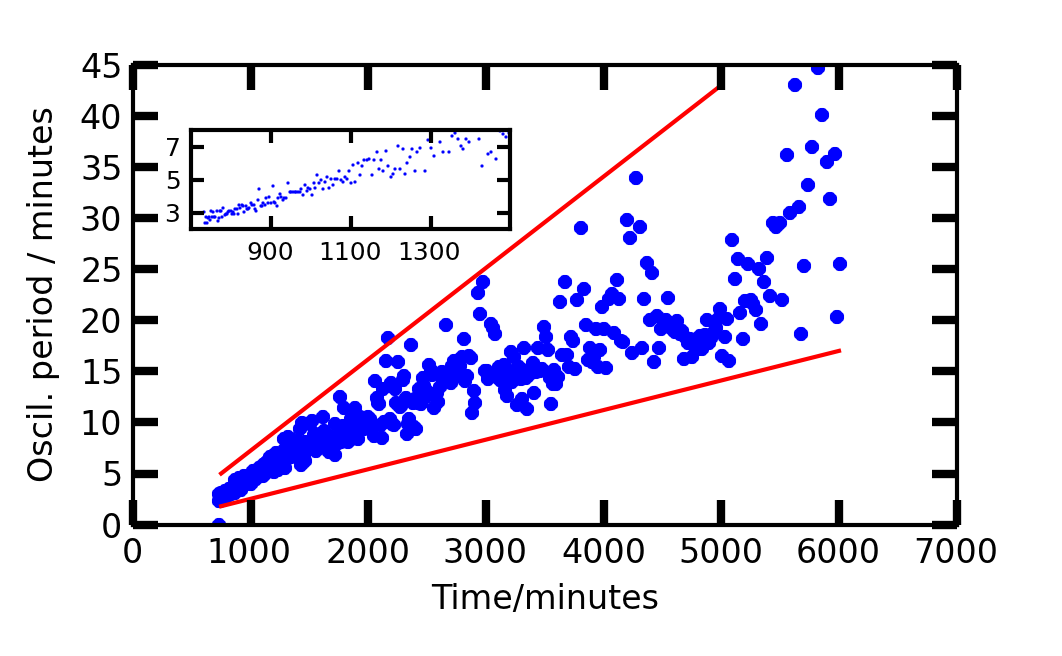
\includegraphics[height=7cm]{summary_of_long_measurement.png}
  \caption{Summary of a sample oscillating under constant temperature, pressure and reactant composition. The sample a total for 439 oscillations in 4 days.}
  \label{fgr:long_measurement}
\end{figure}

Extracts of the mass-spectrometry from the very beginning, the middle and towards the end of the experiments is shown in figure~\ref{fgr:extracts}, it is evident that the oscillations are getting more and more irregular as times goes on, towards the end, it is also clearly visible how the smaller oscillations are taking place at a much higher frequency than the full on-off cycles, which is most likely the explanation for the increasing scatter in the period summary.
% an example of a two-column figure, remember that the graphics should be included where it is first referenced
\begin{figure*}
  \centering
  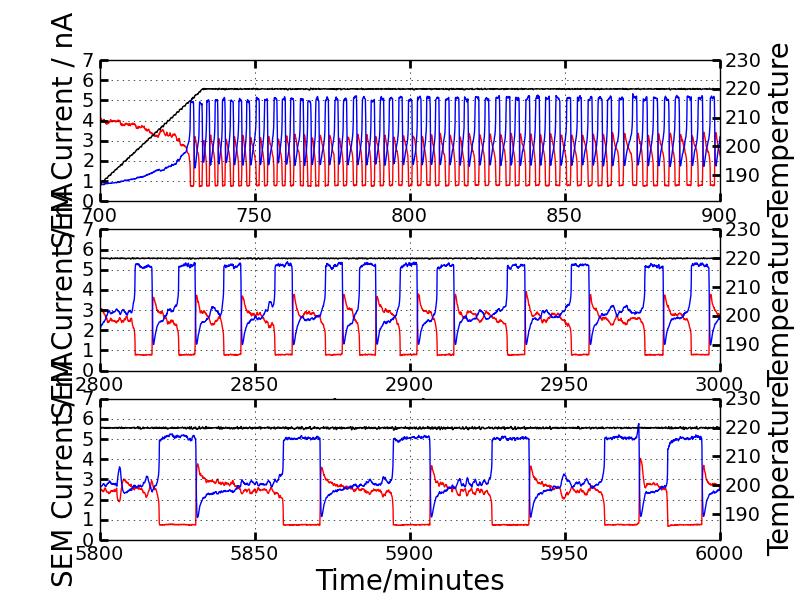
\includegraphics[height=7cm]{extracts_from_very_long_oscillation.png}
  \caption{Extracts from the 4 day long experiment.}
  \label{fgr:extracts}
\end{figure*}



Several different samples deposited at various diffent sizes and amounts all show the oscillating bahaviour. Repeatability is high regarding running long experiments on a single sample, but very low from sample to sample.

\section{Discussion}
Due to long timescales involved which are much larger than any typically orcurring timescales for such a small system, there can be little doubt that this phenomenon involves some kind of reaction involving the bulk of the nano particles.




%\subsection{This is the subsection heading style}
%Section headings can be typeset with and without numbers.\cite{Gong2004} \cite{Hendriksen2010}

%\subsubsection{This is the subsubsection style.~~} These headings should end in a full point.  

%\paragraph{This is the next level heading.~~} For this level please use \texttt{\textbackslash paragraph}. These headings should also end in a full point.

\section{Equations}

Equations can be typeset inline \textit{e.g.} $ y = mx + c$ or displayed with and without numbers:

 \[ A = \pi r^2 \]

\begin{equation}
  \frac{\mathrm{\gamma}}{\mathrm{\epsilon}x} r^2 = 2r
\end{equation}

\section{Graphics and tables}
\subsection{Graphics}
Graphics should be inserted on the page where they are first mentioned (unless they are equations, which appear in the flow of the text).



\subsection{Tables}
Tables typeset in RSC house style do not include vertical lines. Table footnote symbols are lower-case italic letters and are typeset at the bottom of the table. Table captions do not end in a full point.


\begin{table}[h]
\small
  \caption{\ An example of a caption to accompany a table}
  \label{tbl:example}
  \begin{tabular*}{0.5\textwidth}{@{\extracolsep{\fill}}lll}
    \hline
    Header one/units & Header two & Header three \\
    \hline
    1 & 2 & 3 \\
    4 & 5 & 6 \\
    7 & 8 & 9 \\
    10 & 11 & 12 \\
    \hline
  \end{tabular*}
\end{table}

Adding notes to tables can be complicated.  Perhaps the easiest
method is to generate these manually.

% an example of a two-column table
%\begin{table*}
%\small
  %\caption{\ An example of a caption to accompany a table, table captions do not end in a full point}
  %\label{tbl:example}
  %\begin{tabular*}{\textwidth}{@{\extracolsep{\fill}}lllllll}
    %\hline
    %Header one & Header two & Header three & Header four & Header five & Header six  & Header seven\\
    %\hline
    %1 & 2 & 3 & 4 & 5 & 6  & 7\\
    %8 & 9 & 10 & 11 & 12 & 13 & 14 \\
    %15 & 16 & 17 & 18 & 19 & 20 & 21\\
    %\hline
  %\end{tabular*}
%\end{table*}

You can also put lists into the text. You can have bulleted or numbered lists of almost any kind. 
The \texttt{mhchem} package can also be used so
that formulae are easy to input: \texttt{\textbackslash ce\{H2SO4\}} gives \ce{H2SO4}. 


\section{Conclusions}
The conclusions section should come at the end of article. For the reference section, the style file rsc.bst can be used to generate the correct reference style.\footnote[4]{Footnotes should appear here. These might include comments relevant to but not central to the matter under discussion, limited experimental and spectral data, and crystallographic data.}
 %For footnotes in the main text of the article please number the footnotes to avoid duplicate symbols. e.g.  \footnote[num]{your text} the corresponding author \ast counts as footnote 1, ESI as footnote 2, e.g. if there is no ESI, please start at [num]=[2], if ESI is cited in the title please start at [num]=[3] etc. Please also cite the ESI within the main body of the text using \dag.





%The \balance command can be used to balance the columns on the final page if desired. It should be placed anywhere within the first column of the last page.

%\balance

%If notes are included in your references you can change the title from 'References' to 'Notes and references' using the following command:
%\renewcommand\refname{Notes and references}

\footnotesize{
\bibliography{literature} %your .bib file
\bibliographystyle{rsc} %the RSC's .bst file
}

\end{document}
